\documentclass[a4paper,UTF8]{article}
\usepackage{ctex}
\usepackage[margin=1.25in]{geometry}
\usepackage{color}
\usepackage{graphicx}
\usepackage{amssymb}
\usepackage{amsmath}
\usepackage{amsthm}
%\usepackage[thmmarks, amsmath, thref]{ntheorem}
\theoremstyle{definition}
\newtheorem*{solution}{Solution}
\newtheorem*{prove}{Proof}
\usepackage{multirow}
\usepackage{url}
% 设置linkcolor为黑色,urlcolor为蓝色
\usepackage[colorlinks,linkcolor=black,urlcolor=blue]{hyperref}
\usepackage{enumerate}
\title{\textbf{系统使用说明书}}
\author{XXX,XXX,211240045@smail.nju.edu.cn}

\begin{document}
	\maketitle
	\tableofcontents 
	\newpage
	
	\section{开发环境}
	
		\subsection{所使用的操作系统}
		Ubuntu 22.04.4 LTS
	
		\subsection{所使用IDE的版本}
		PyCharm 2023.3
	
		\subsection{python的版本}
		Python 3.10
	
		\subsection{python库的版本}
		PyQt5 5.15.10
	
		PyQt5-Qt5 5.15.2
	
		PyQt5-sip 12.13.0
	
		PyQt5-stubs 5.15.6.0
	
		numpy 1.26.4
	
		pillow 10.2.0
	
		pip 24.0
	
		setuptools 69.1.1
	
		wheel 0.42.0
	
	\section{功能介绍}
		\subsection{文件功能}
		\subsubsection{设置画笔}
		点击“文件”,点击“设置画笔”,在弹出的对话框中设置画笔的颜色即可。
		\begin{center}
			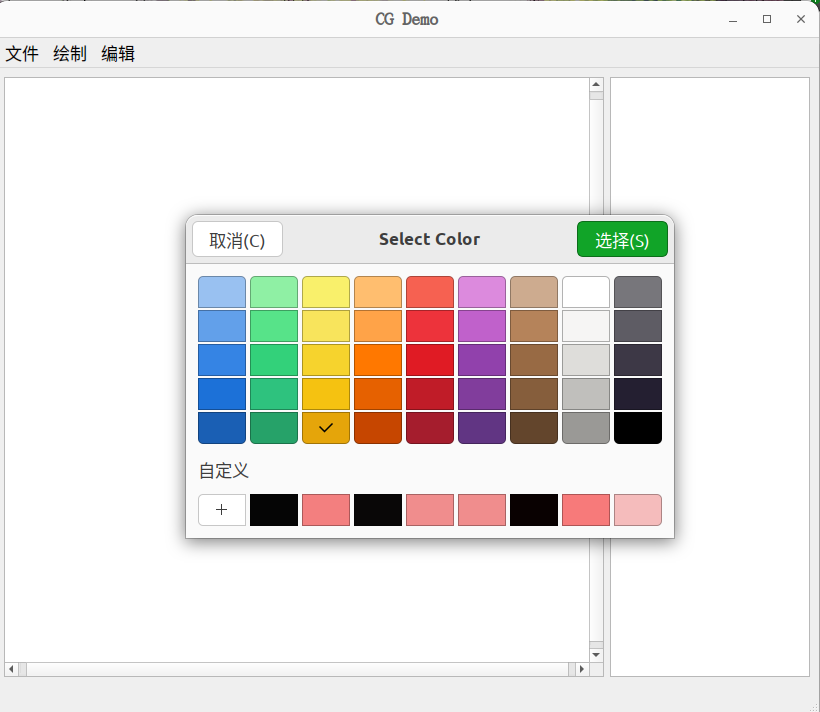
\includegraphics[width=5in]{说明书/1.png}
			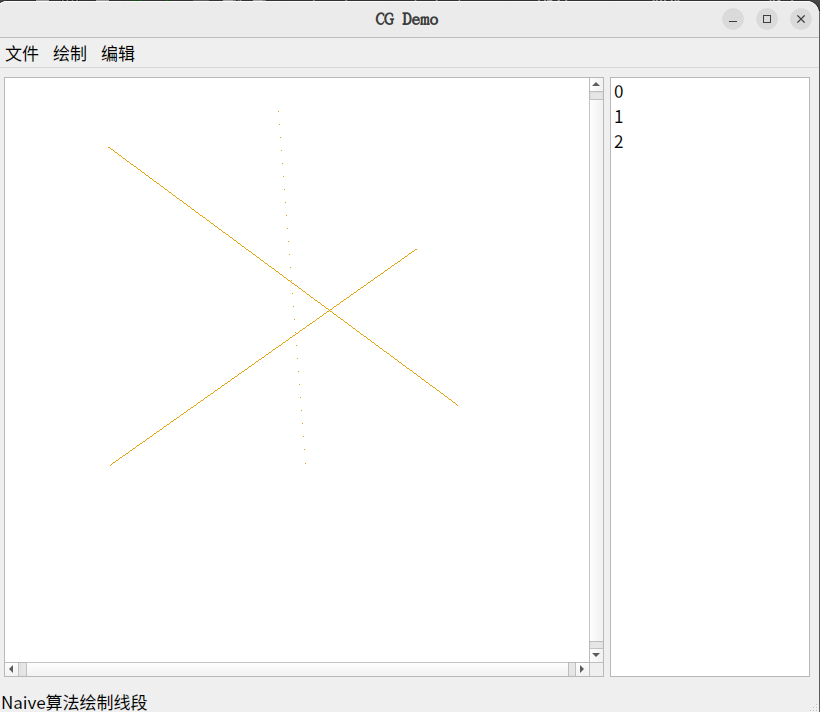
\includegraphics[width=5in]{说明书/2.png}
		\end{center}
	
		\subsubsection{重置画布}
		点击“文件”,点击“重置画布”,在弹出的对话框中给定新画布的height和width即可。
		\begin{center}
			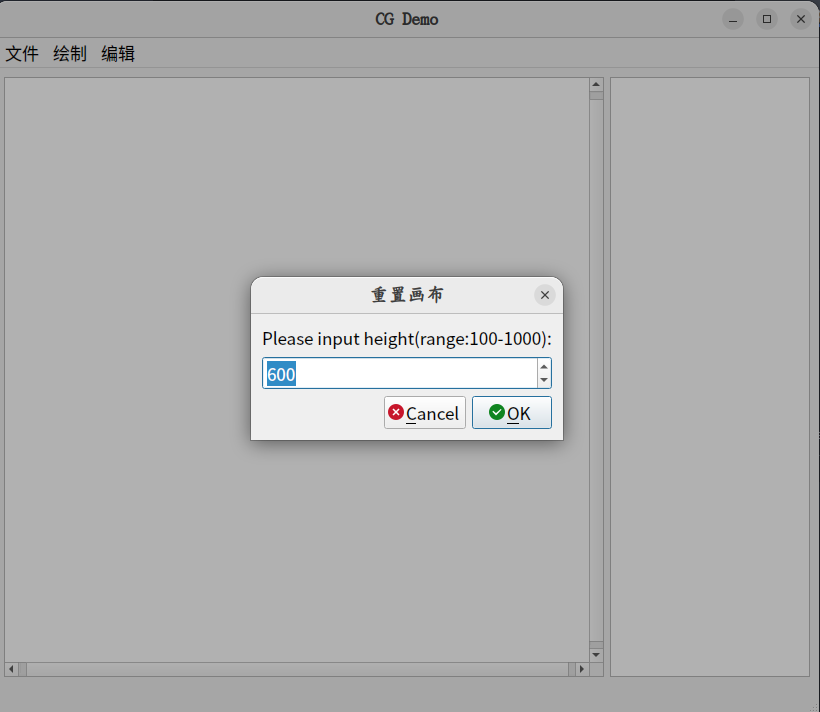
\includegraphics[width=5in]{说明书/3.png}
		\end{center}
	
		\subsubsection{保存画布}
		点击“文件”,点击“保存画布”,在弹出的对话框中给定保存后图像的文件路径和文件名即可,支持.jpg/.png/.bmp格式的文件。保存的“ellipse.bmp“在saved\_files/目录下。
		\begin{center}
			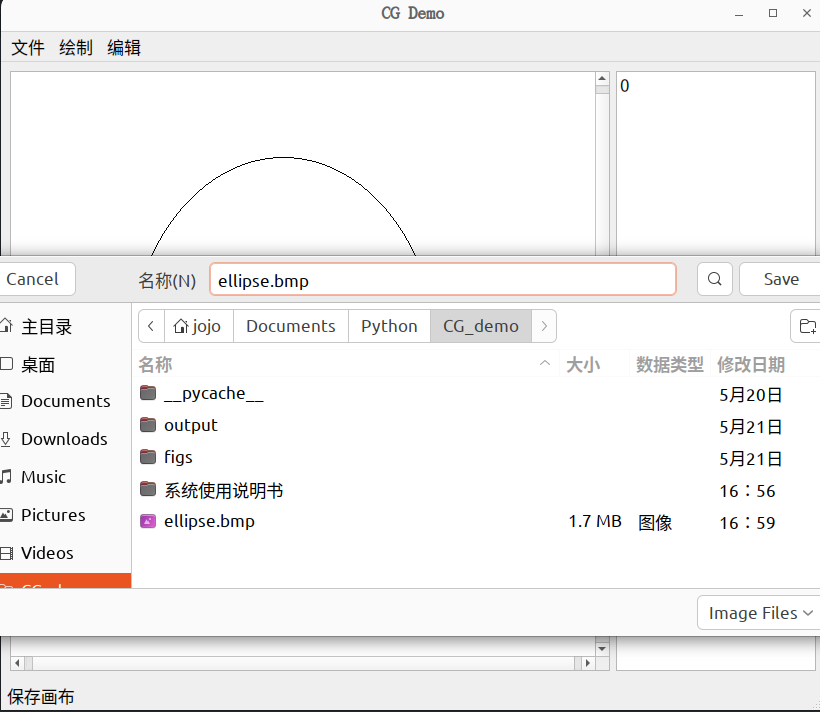
\includegraphics[width=5in]{说明书/4.png}
		\end{center}
	
		\subsubsection{退出}
		点击“文件”,点击“退出”,即可退出当前系统。
		
		\subsection{绘制功能}
		\subsubsection{绘制直线}
		点击“绘制”,鼠标移动悬浮在“线段”上,在弹出的文本框中选择对应的直线绘制算法即可开启直线绘制功能,支持的直线绘制算法有Naive, DDA, Bresenham三种。如下图,最左侧的直线是Naive方法绘制的直线,中间的直线是DDA算法绘制的直线,最右侧的直线是Bresenham算法绘制的直线。
		
		在绘制直线功能开启后,鼠标在画布上按下时确定直线的起点,后随着鼠标移动将动态更新直线的终点,最后释放鼠标时确定直线的终点,直线绘制完成。
		\begin{center}
			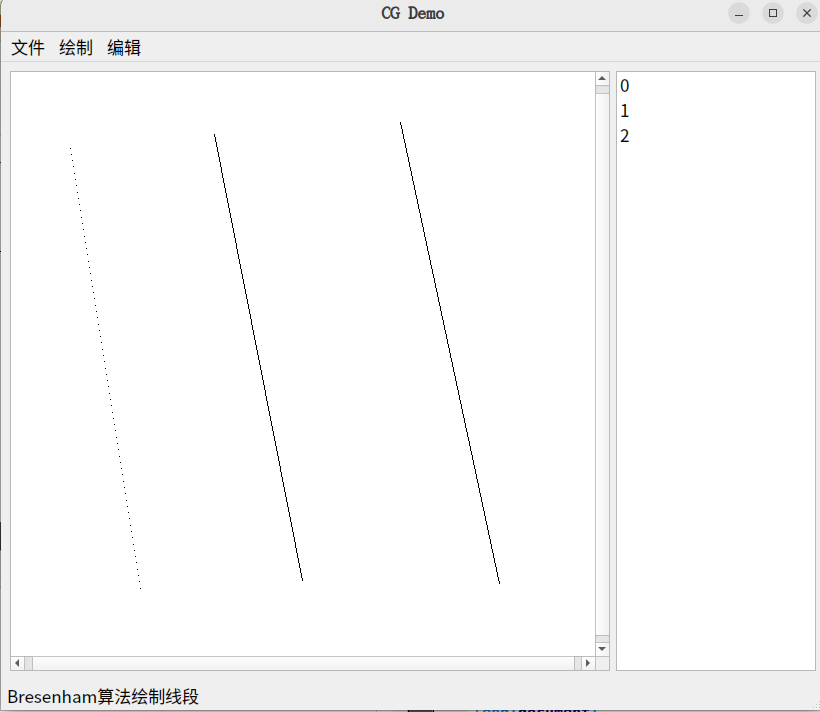
\includegraphics[width=5in]{说明书/5.png}
		\end{center}
		
		\subsubsection{绘制多边形}
		点击“绘制”,鼠标移动悬浮在“多边形”上,在弹出的文本框中选择对应的多边形绘制算法即可开启多边形绘制功能,支持的多边形绘制算法有DDA, Bresenham两种。如下图,左侧的多边形是DDA算法绘制的多边形,右侧的多边形是Bresenham算法绘制的多边形。
		
		在绘制多边形功能开启后,鼠标在画布上点击一次即确定多边形的一个端点,当新加入的点与第一个点的曼哈顿距离小于10时,该新加入的点不构成多边形的端点集,而视为多边形绘制完成的标志。
		\begin{center}
			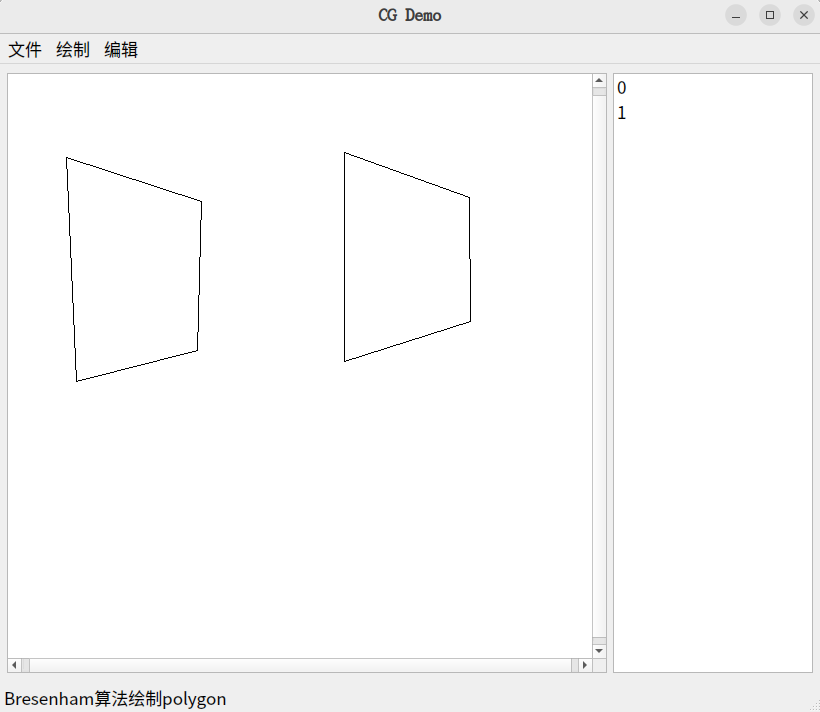
\includegraphics[width=5in]{说明书/6.png}
		\end{center}
	
		\subsubsection{绘制椭圆}
		点击“绘制”,点击“椭圆”,即可开启椭圆绘制功能。
		
		在绘制椭圆功能开启后,鼠标在画布上按下时确定椭圆外接矩形一条对角线的起点,后随着鼠标移动动态更新该对角线的终点,最后释放鼠标时确定该对角线的终点,椭圆被唯一确定,椭圆绘制完成。
		\begin{center}
			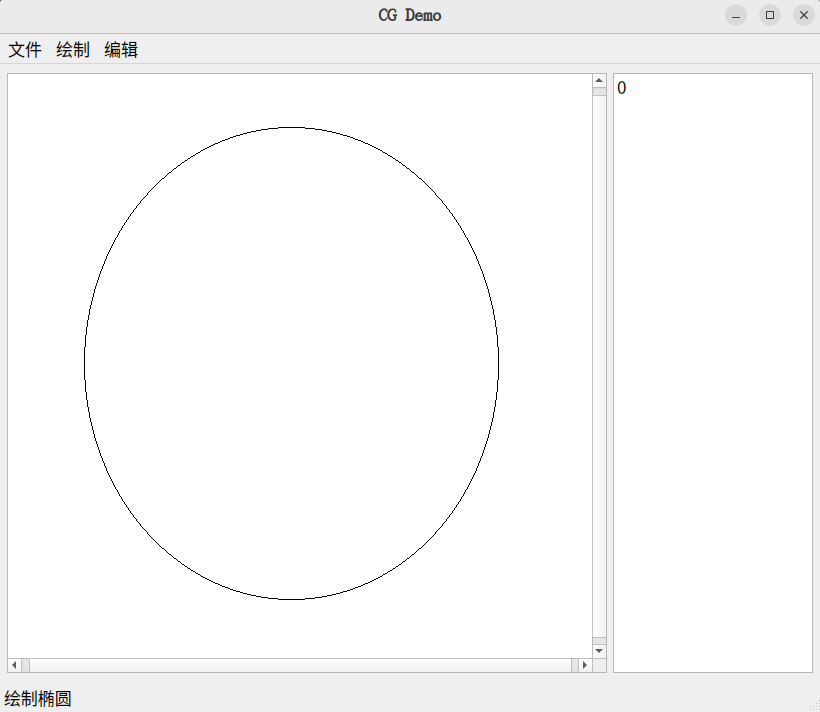
\includegraphics[width=5in]{说明书/7.png}
		\end{center}
		
		\subsubsection{绘制曲线}
		点击“绘制”,鼠标移动悬浮在“曲线”上,在弹出的文本框中选择对应的曲线绘制算法即可开启曲线绘制功能,支持的曲线绘制算法有Bezier, B-spline两种。如下图,左侧的曲线是Bezier算法绘制的曲线,右侧的曲线是B-spline算法绘制的多边形。
		
		Bezier算法下,鼠标在画布上第一次点击确定曲线的起点,第二次点击确定一有效控制顶点,第三次点击确定曲线的终点。B-spline算法下,手册要求绘制三次(四阶)均匀B样条曲线,同样三次点击确定曲线。
		\begin{center}
			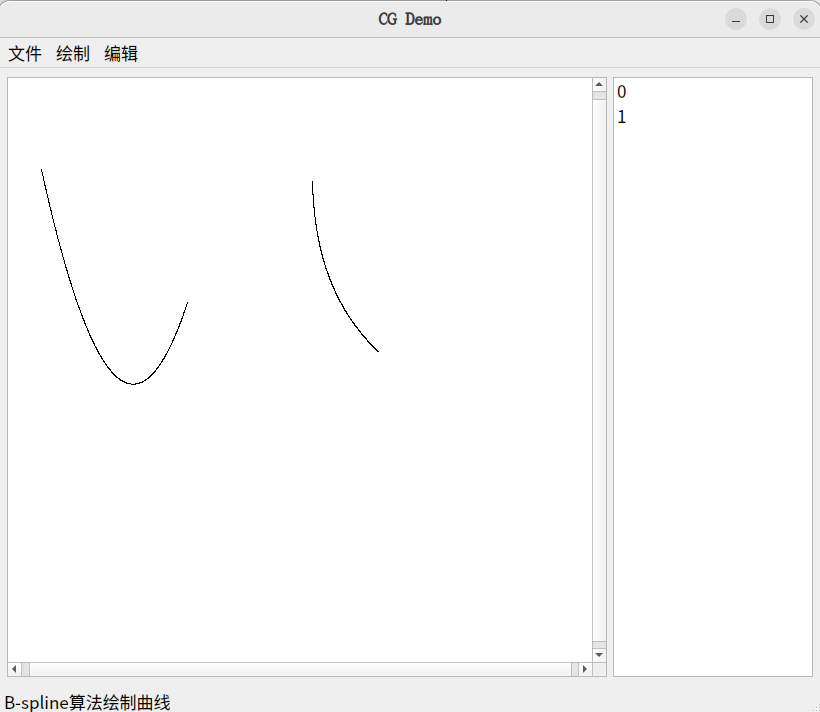
\includegraphics[width=5in]{说明书/8.png}
		\end{center}
	
		\subsection{编辑功能}
		\subsubsection{平移}
		先在右边的选择栏中选择需要进行平移的图元,然后点击“编辑”,点击“平移”,即可开启平移功能。此时在画布上按下鼠标确定平移起点,后随着鼠标移动动态更新平移终点,最后释放鼠标完成平移过程。
		\begin{center}
			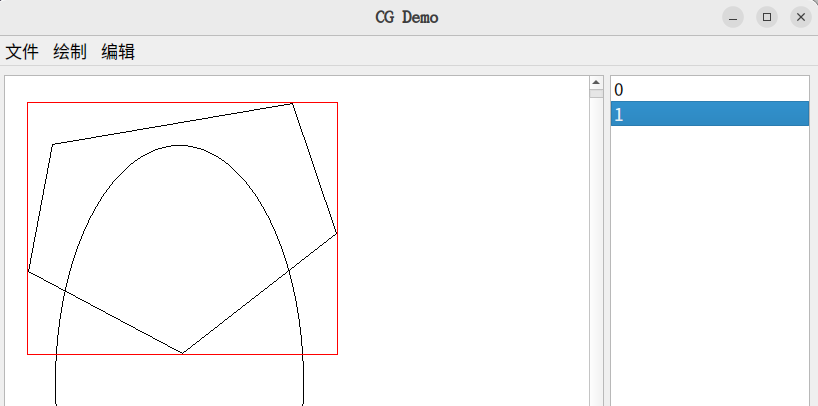
\includegraphics[width=5in]{说明书/9.png}
			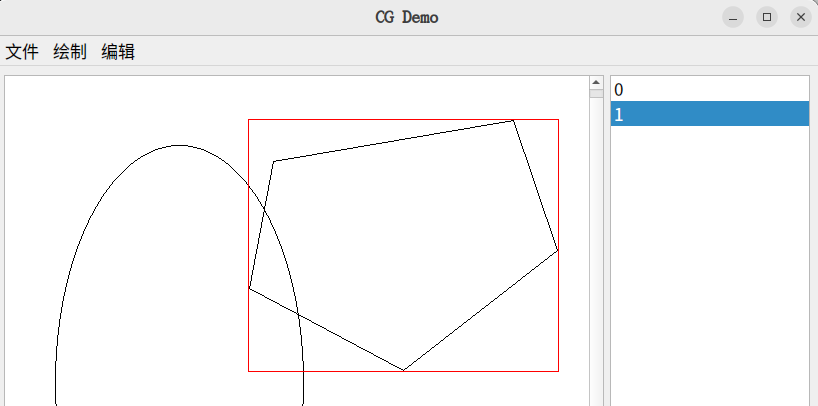
\includegraphics[width=5in]{说明书/10.png}
		\end{center}
	
		\subsubsection{旋转}
		先在右边的选择栏中选择需要进行旋转的图元,然后点击“编辑”,点击“旋转”,即可开启旋转功能。此时在画布上按下鼠标确定旋转起点,后随着鼠标移动动态更新旋转角度,最后释放鼠标完成旋转过程。
		\begin{center}
			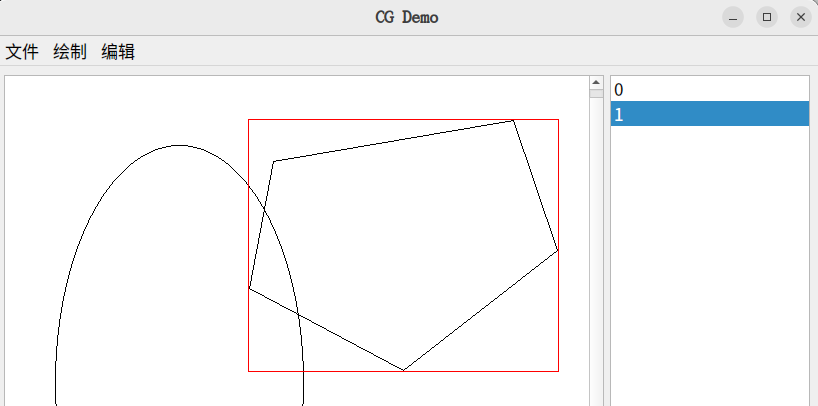
\includegraphics[width=5in]{说明书/10.png}
			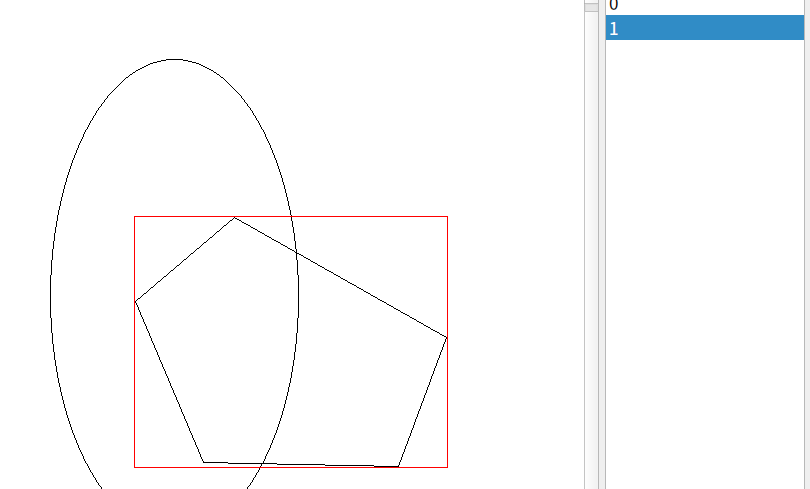
\includegraphics[width=5in]{说明书/11.png}
		\end{center}
		
		\subsubsection{缩放}
		先在右边的选择栏中选择需要进行缩放的图元,然后点击“编辑”,点击“缩放”,即可开启缩放功能。此时在画布上按下鼠标确定缩放起点,后随着鼠标移动动态更新缩放因子,最后释放鼠标完成缩放过程。
		\begin{center}
			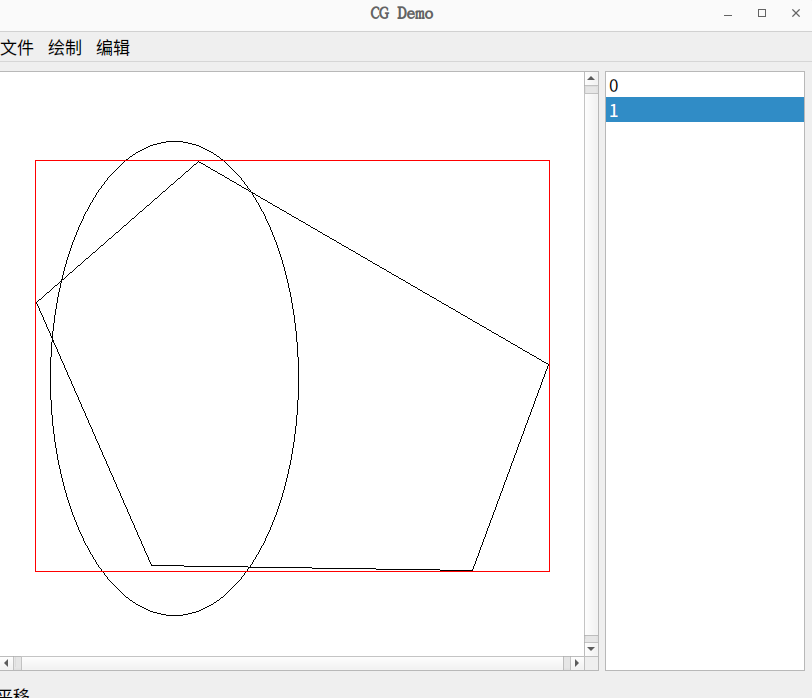
\includegraphics[width=5in]{说明书/12.png}
		\end{center}
	
		\subsubsection{线段裁剪}
		先在右边的选择栏中选择需要进行裁减的直线图元,然后点击“编辑”,将鼠标悬浮于“裁减”上,在弹出的文本框中选择对应的线段裁减算法即可开启线段裁减功能,支持的线段裁减算法有Cohen-Sutherland算法和Liang-Barsky算法两种。如下图,上侧的线段经Cohen-Sutherland算法进行裁减,下侧的线段经Liang-Barsky算法进行裁减。
		
		在裁减功能开启后,鼠标在画布上按下时确定裁剪窗口一条对角线的起点,后随着鼠标移动动态更新该对角线的终点,也就是动态更新裁减窗口的位置和大小,最后释放鼠标时确定该对角线的终点,裁减窗口被唯一确定,裁减功能完成。
		\begin{center}
			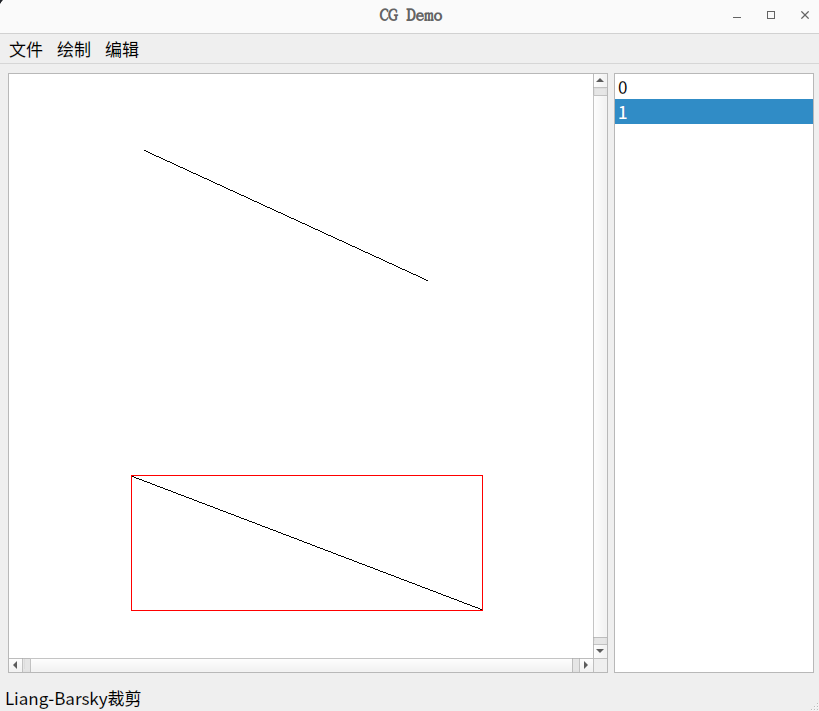
\includegraphics[width=5in]{说明书/13.png}
		\end{center}
\end{document}